\documentclass[10pt,a4paper]{article}
\usepackage[margin=17mm]{geometry}
\usepackage{fontspec,amsmath,graphicx,booktabs,array}
\setmainfont{Latin Modern Roman}
\setlength{\parindent}{0pt}\setlength{\parskip}{6pt}
\begin{document}
{\LARGE Ordered arc-length matching}\hfill 6 October 2026

Three models, two intervals; fixed optics and intensity objective. Equal-arc matching uses one cyclic offset and tests both directions, preserving the order through both loops. Flexible controls retain the 16 phase parameters. Both are fitted anew to the same calibrated bins.

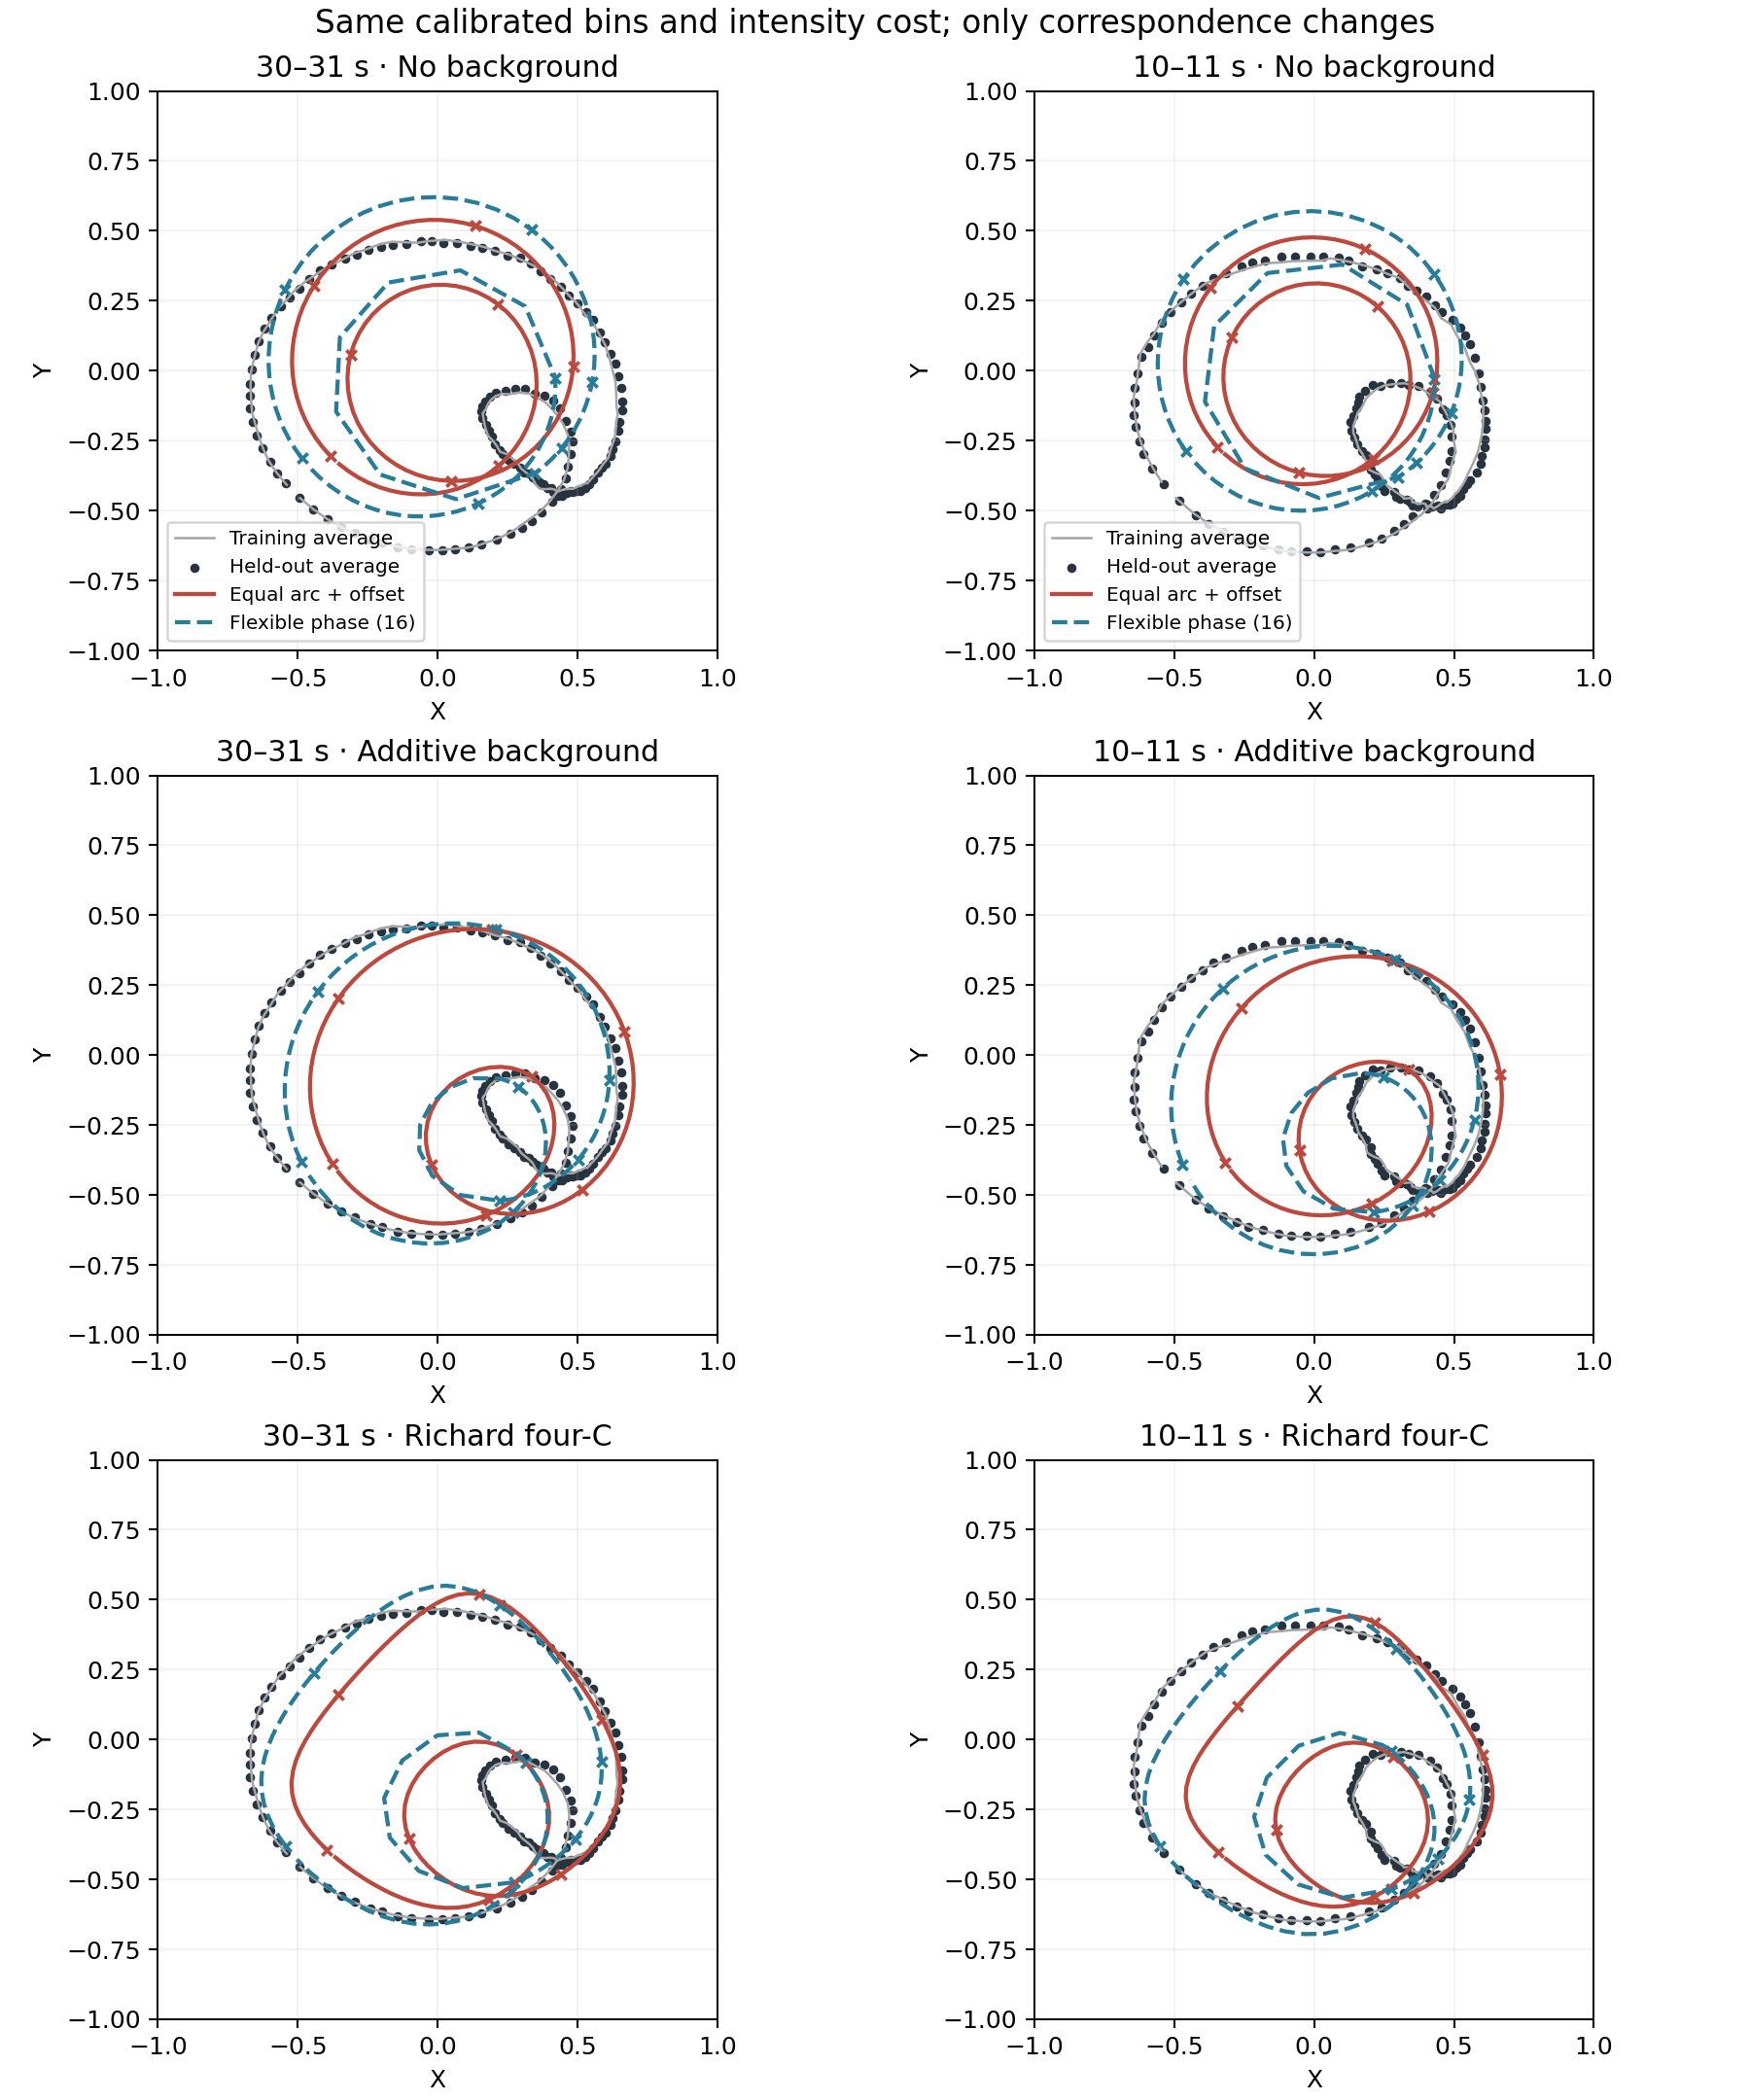
\includegraphics[width=\linewidth,height=.84\textheight,keepaspectratio]{arc_comparison.png}
\newpage
{\Large Quantitative comparison}

Errors below are held-out scores. Channel RMS is dimensionless: each channel residual is divided by the observed total intensity at that bin. XY RMS is an additional diagnostic, not the fitted objective.

\begin{tabular}{llrrrr}\toprule
Window & Model / matching & Channel RMS & XY RMS & BG/\(T_{\max}\) & \(\theta\) range\\\midrule
30s & No background / arc & 0.06726 & 0.34194 & 0.0\% & 33.4--48.2$^\circ$ \\
30s & No background / flex & 0.03927 & 0.17830 & 0.0\% & 37.0--53.5$^\circ$ \\
30s & Additive background / arc & 0.02990 & 0.14642 & 34.1\% & 37.8--90.0$^\circ$ \\
30s & Additive background / flex & 0.02292 & 0.08981 & 31.9\% & 37.1--89.5$^\circ$ \\
30s & Richard four-C / arc & 0.03641 & 0.16645 & --- & 36.6--74.6$^\circ$ \\
30s & Richard four-C / flex & 0.02560 & 0.10385 & --- & 36.5--72.1$^\circ$ \\
10s & No background / arc & 0.06984 & 0.35358 & 0.0\% & 33.8--44.2$^\circ$ \\
10s & No background / flex & 0.04308 & 0.18240 & 0.0\% & 38.6--50.2$^\circ$ \\
10s & Additive background / arc & 0.03146 & 0.15442 & 37.1\% & 37.6--90.0$^\circ$ \\
10s & Additive background / flex & 0.02566 & 0.09880 & 34.8\% & 41.8--90.0$^\circ$ \\
10s & Richard four-C / arc & 0.03827 & 0.17479 & --- & 40.1--73.6$^\circ$ \\
10s & Richard four-C / flex & 0.02716 & 0.10538 & --- & 40.1--71.5$^\circ$ \\
\bottomrule\end{tabular}

Richard's model does not infer physical background power; a dash does not mean zero background. Its effective correction is \(C_i\sqrt{S_i}\), with one constant signed \(C_i\) per channel per interval.

\textbf{Result.} Both background hypotheses improve substantially over no background. Equal-arc correspondence gives poorer held-out four-channel and XY agreement than flexible phase on both intervals. Additive equal-arc fits do give smaller total-intensity residuals, so the difference includes a trade-off between intensity balance and anisotropy shape. Neither correspondence is validated against known rod angles.

\textbf{Sampling controls.} Original gate crossings were retained (304 and 217 complete traversals). Arc bins were rebuilt using calibrated channel ratios. All observed bin intensities are means of unsmoothed calibrated samples. Alternating traversals form training and held-out averages, with equal weight per traversal. The flexible results remain close to the preceding raw-guide-bin results.

\textbf{Numerical and averaging checks.} Increasing simulated curve resolution from 2048 to 8192 segments changes predicted channel intensities by no more than \(1.02\times10^{-6}T_{\max}\) in these selected arc fits. Averaging predictions over the empirical within-bin dwell distributions and refitting changes held-out channel RMS by less than 0.000012 and pointwise folded theta by less than \(0.024^\circ\). Thus neither midpoint approximation nor numerical resolution explains the larger correspondence difference. Dwell coordinates come from the smoothed measured guide, not independent true orientations.

\textbf{Optimization checks.} Arc fits used 20--21 starts per model/window, both directions. Flexible controls used 9--10 starts, including an arc-derived start. All selected runs converged, selected full arc curves have positive channel intensities, and multiple starts found the reported minima. These are local-search results, not certified global minima. Expanded models were seeded with the fitted zero-background solution and obey the nested training-cost bound.

\newpage
{\Large Recovered angles and model definition}

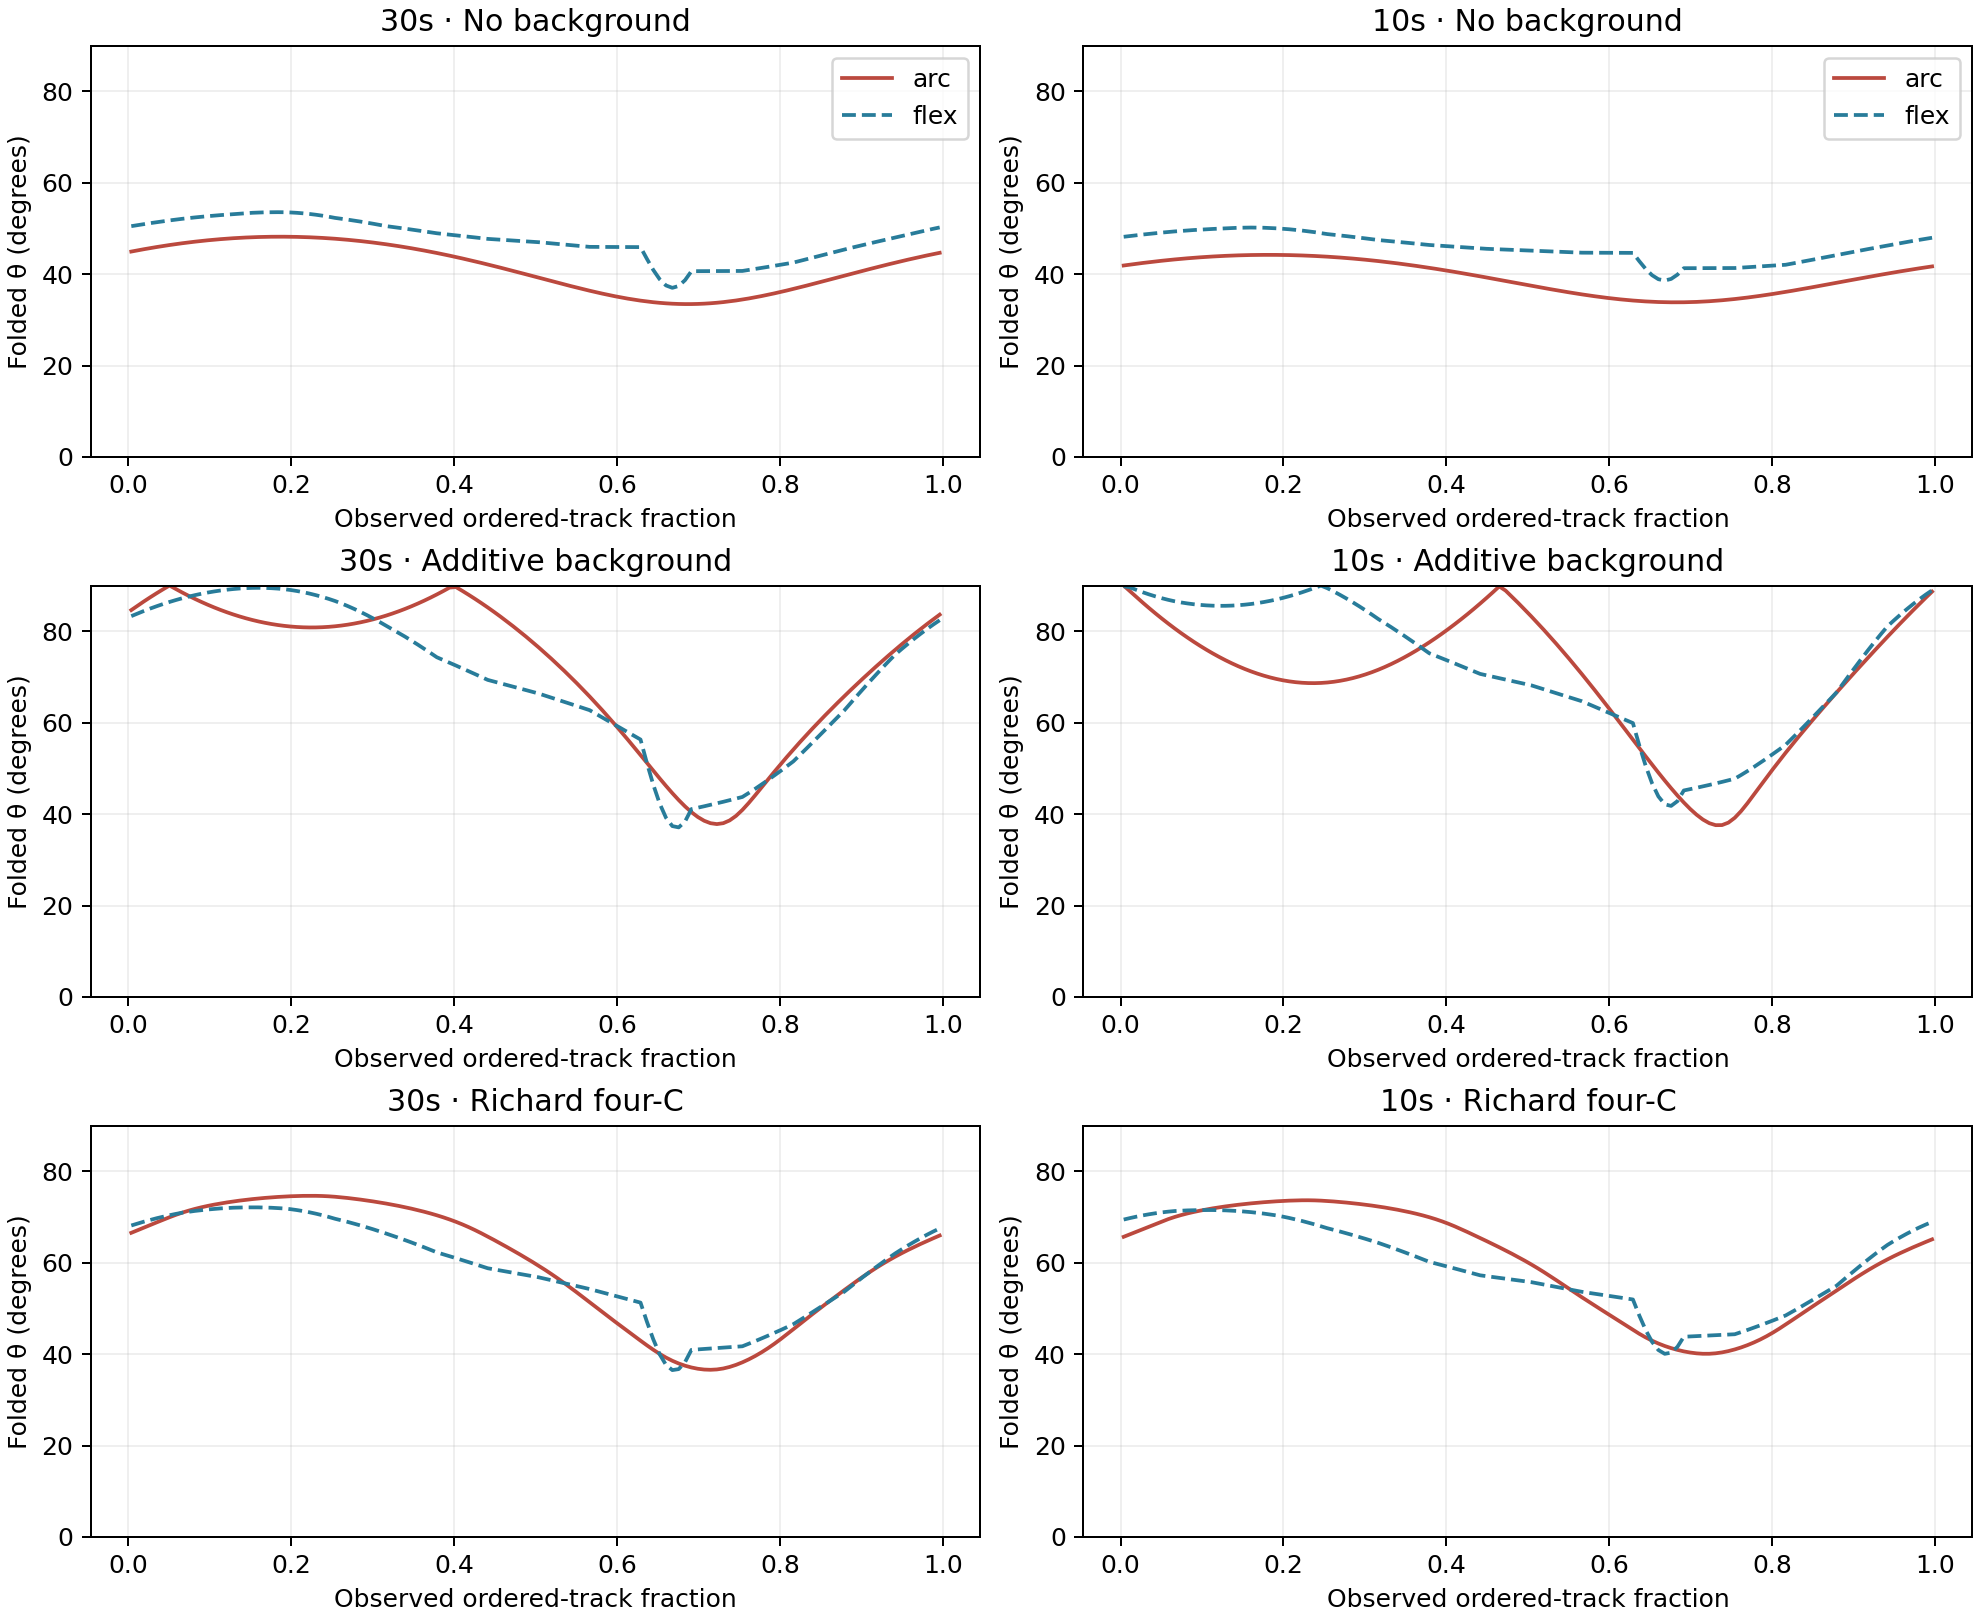
\includegraphics[width=\linewidth]{angles.png}

For \(q_i=A_F+B_F\sin^2\theta+C_F\sin^2\theta\cos2(\phi-\psi_i)\),
\[
S_i=a_0^2\sin^2\theta\,q_i,
\qquad I_i^{\rm pred}=\begin{cases}S_i&\text{none},\\ S_i+B_i&\text{additive},\\S_i+C_i\sqrt{S_i}&\text{Richard}.
\end{cases}
\]
\[
B_i=\frac{B_{\rm total}}4(1+f_a,1-f_a,1+f_b,1-f_b)_i,
\quad f_a,f_b\in[-1,1],\quad B_{\rm total}\leq0.95\min T_{\rm train}.
\]
Equal-arc matching evaluates this full model densely, forms measured-model X/Y, integrates its arc length, and interpolates the four intensities at ordered fractions plus one cyclic offset. No independent nearest-point matches are made. Cone geometry, brightness and correction parameters are jointly fitted using
\[
J=\sum_{k,i}\left(\frac{I_{i,k}^{\rm pred}-I_{i,k}^{\rm obs}}{T_k^{\rm obs}}\right)^2.
\]
Parameters: 5/8/9 for equal arc; 20/23/24 for flexible phase. Angles here follow each fitted cone; they are not independent angle measurements. Folding near 90 degrees can create cusps in the displayed traces.
\end{document}
